\chapter{INTRODUCTION}
\label{chap-one}

\section*{Introduction}

This Chapter provides an introduction into sound propagation in porous materials.

\section{Motivation}

The study of acoustic properties of porous materials has been of interest in many research publications in recent years \cite{Horoshenkov2013}. Noise pollution is considered to be a major health concern in both homes and places of employment. It has been shown that exposure to large durations and magnitudes of sound results in permanent loss of hearing and damage to cells \cite{Bohne2007}. A means of solving this issue is the use of absorption materials to provide control over the acoustics in a given environment. Noise control solutions have a broad range of applications such as the industrial, automotive, architectural and medical fields. \cite{Beranek1969} \cite{Shoureshi1996} \cite{Horoshenkov2013}. In recent years, environmentally and biologically friendly materials have gained interest as a research subject. \cite{Ersoy2009} \cite{Wassilieff1996}. Currently, the sound absorption market is dominated with glass wool, foam and fibrous materials which prove to be the most valuable materials. However, many of these materials are not the best suited for close contact with humans. For example, fiberglass which is a common absorption material, has hazardous effects when ingested by an individual. For this reason, biologically friendly porous materials as alternatives to current solutions are of interest. An advantage to these materials is that they allow for sound damping in desirable, however previously unfeasible locations and applications such as dampening in the medical setting.

\section{Applications}

\subsection{Acoustics}
The ability to control the sound pressure levels in a room is desirable to engineers, architects and acousticians alike. Modern day architecture goes to great lengths to consider the level of noise pollution in a space. This ranges from industrial, automotive, musical, and education space applications. It also has a wide range of practical uses in daily life. \cite{Beranek1969} \cite{Shoureshi1996}.

In general, there exist various acoustic treatments which need to be considered when designing the acoustic space in a room. The treatments focus on absorption, reflection and diffusion \cite{Cox2004}. Figure \ref{fig:acoustictreaments} shows how each of these vary. The focus for noise controllability is the absorption treatment. The ability to control noise stems from 3 key principles. These are absorption, specular reflection and diffuse reflection as can be seen in Figure \ref{fig:noisecontrol}. Absorption is the key variable. 

% Acoustic Treatments
\begin{figure}[hbtp]
    \centering
    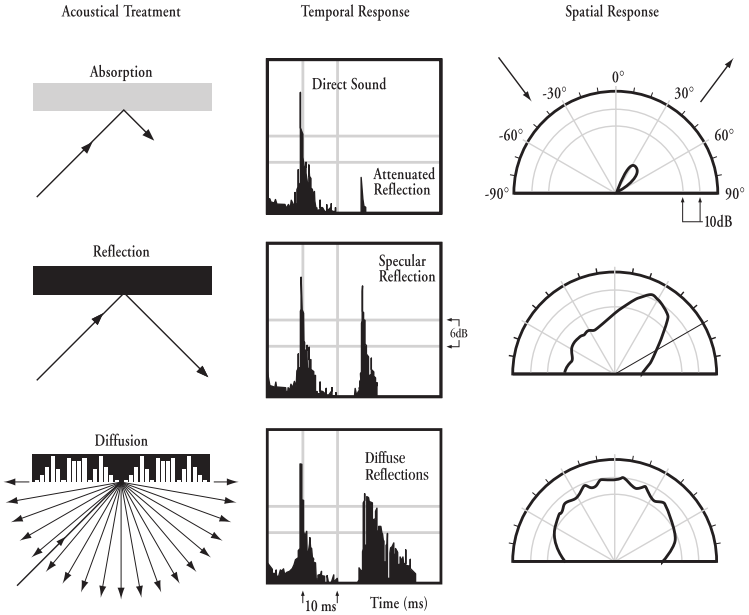
\includegraphics[width=1\textwidth]{Chapter-1/figs/acoustictreaments}
    \caption{Acoustic Treatments \cite{Cox2004}}
    \label{fig:acoustictreaments}
\end{figure}

% Noise Control
\begin{figure}[hbtp]
    \centering
    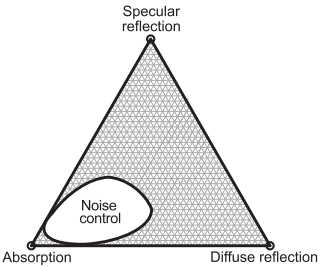
\includegraphics[width=0.7\textwidth]{Chapter-1/figs/noisecontrol}
    \caption{Breakdown of Noise Control \cite{Cox2004}}
    \label{fig:noisecontrol}
\end{figure}

\clearpage

Usually, acoustic absorption is broken down into two types. These are active absorption and passive absorption. Generally, active noise control solutions perform better in low frequencies while passive noise control solutions perform better in higher frequencies as shown in Figure \ref{fig:passivevsactive}. Absorbing materials are passive mediums that lower noise by disseminating energy and turning energy into heat. In porous materials at high frequencies, an adiabatic process takes places that produces heat loss due to friction when the sound waves cross the uneven pores. At lower frequencies poroelastic materials absorb sound by energy loss caused by heat exchange. This is an isothermal process. This is why poroelastic materials are much more efficient at absorbing higher frequencies \cite{Sagartzazu2008}.
% Active vs. Passive frequency ranges
\begin{figure}[hbtp]
    \centering
    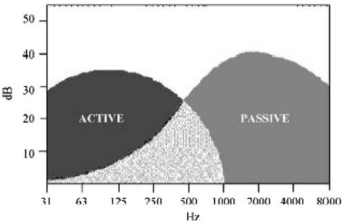
\includegraphics[width=0.6\textwidth]{Chapter-1/figs/passivevsactive}
    \caption{Active vs. Passive Noise Control frequencies \cite{Sagartzazu2008}}
    \label{fig:passivevsactive}
\end{figure}

Figure \ref{fig:activeNoiseComplex} shows an automotive application control system. However, it is noted that these systems require input energy and are generally very complex \cite{Shoureshi1996}. Passive techniques are generally used in architectual spaces as can be seen in Figure \ref{fig:woodabsorption} and Figure \ref{fig:concerthall}.

% Active Noise Canceling Automotive application Figure!
\begin{figure}[hbtp]
    \centering
    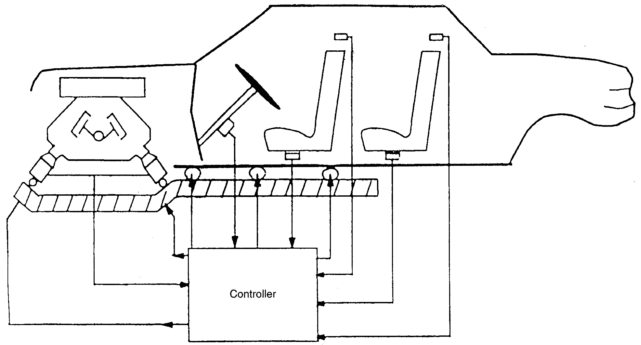
\includegraphics[width=0.8\textwidth]{Chapter-1/figs/activeNoiseComplex}
    \caption{Active Noise Control Application - Automotive \cite{Shoureshi1996}}
    \label{fig:activeNoiseComplex}
\end{figure}

% Passive Example 1
\begin{figure}[hbtp]
    \centering
    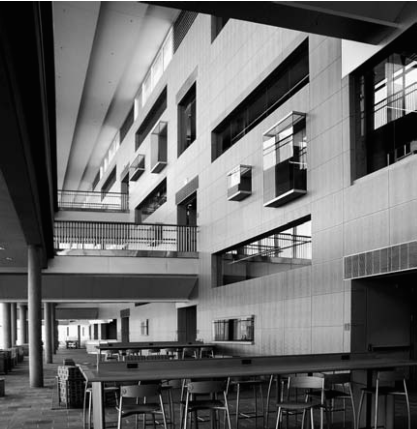
\includegraphics[width=0.5\textwidth]{Chapter-1/figs/woodabsorption}
    \caption{Passive Application - Wooden Architecture \cite{Cox2004}}
    \label{fig:woodabsorption}
\end{figure}

% Passive Example 2
\begin{figure}[hbtp]
    \centering
    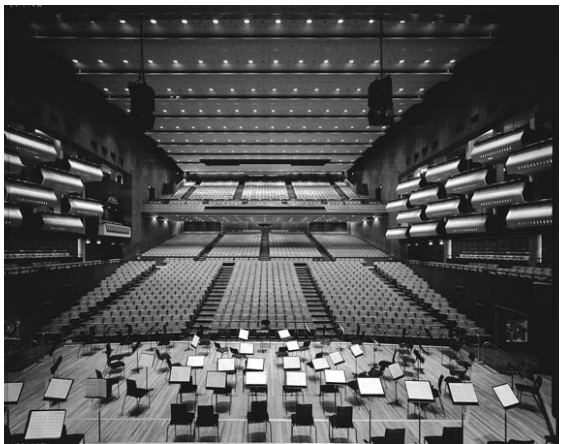
\includegraphics[width=0.55\textwidth]{Chapter-1/figs/concerthall}
    \caption{Passive Application - Concert Hall \cite{Cox2004}}
    \label{fig:concerthall}
\end{figure}

\clearpage

\subsection{Cellulose Acetate}
Cellulose Acetate is the acetate ester of cellulose. Figure \ref{fig:celluloseacetatestructure} shows the chemical structure of Cellulose Acetate. Cellulose Acetate is made by combining cellulose (cotton) and acetic acid. \cite{Welch1924} Cellulose Acetate can be manufactured with various filler materials, and made into different forms. Since cellulose acetate is such a basic chemical, it has a variety of uses outside of acoustics. A commonly known form of cellulose acetate with a TiO$_{\text{2}}$ filler manufactured into rods is the material used in cigarette filters.

% Cellulose Acetate Structure Figure!
\begin{figure}[hbtp]
    \centering
    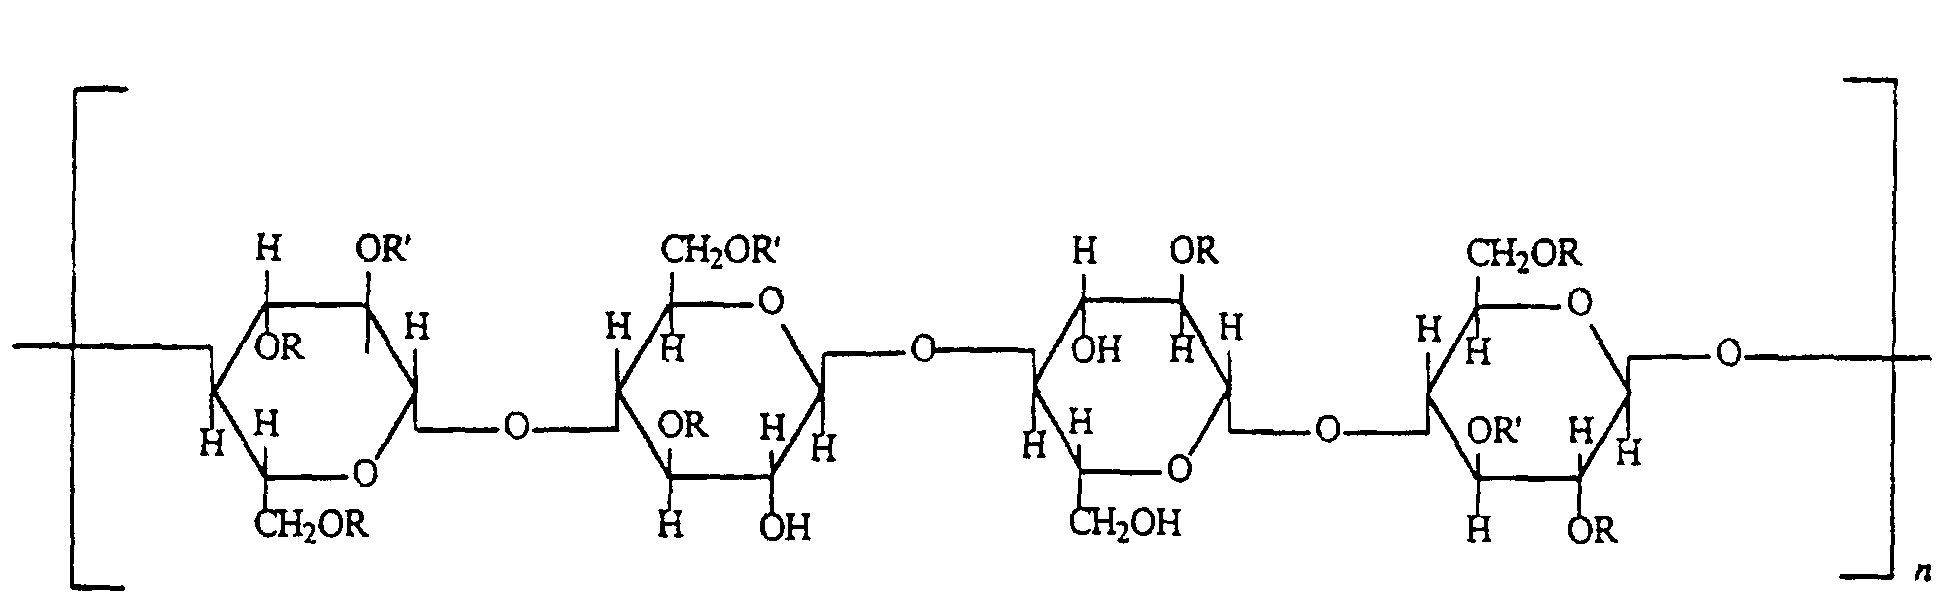
\includegraphics[width=1\textwidth]{Chapter-1/figs/celluloseacetatestructure}
    \caption{General Structure of Cellulose Acetate}% \cite{CA}}
    \label{fig:celluloseacetatestructure}
\end{figure}

\clearpage

Porous materials come in many varieties as shown in Figure \ref{fig:soundabsorbingmaterials}. Parts a) and b) show an SEM image of acoustic foams. Parts c) and d) show fibrous type materials. Cellulose Acetate is able to be manufactured into either of these microstructures.

% Sound absorbing materials Figure!
\begin{figure}[hbtp]
    \centering
    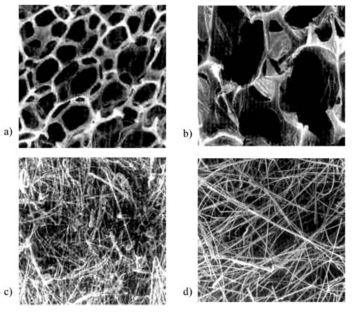
\includegraphics[width=0.8\textwidth]{Chapter-1/figs/soundabsorbingmaterials}
    \caption{Structures of different porous materials: (a) Reticulated foam (b) Partial reticulated foam (c) Mineral Wool (d) Fiberglass \cite{Sagartzazu2008}}
    \label{fig:soundabsorbingmaterials}
\end{figure}

\section{Biocompatibility}

For a new sound absorption material to be competitive in the currently dominated sound absorption market, it must present some novelty. A material that is biologically friendly enables new applications for the control of sound in rooms. Cellulose Acetate has been investigated and does not present health concerns. \cite{Liu2002} \cite{Nguyen2013} \cite{Welch1924} \cite{Zeng2009} 

It is important to note that the Cellulose Acetate Tow used in the experiments in this paper has a TiO$_{\text{2}}$ filler material used in it as manufactured by Eastman Chemical Company. It has been noted by \cite{Welch1924} that it is possible to make Cellulose Acetate with other hazardous chemicals, however the filler TiO$_{\text{2}}$ is not one of these. Therefore the Cellulose Acetate used in the experiments in this paper is biologically friendly.

\section{Previous Work}

Much research in the field of understanding how porous materials function for sound absorption has occurred. Due to the complex nature of the problems, empirical relationships have been developed. Similarly, an investigation into the poroelastic parameters controlling the absorption has occurred. Chapter \ref{chap-two} will discuss previous work in the field of porous absorption, as well as, develop the required equations as they relate to Cellulose Acetate absorption.

\section{Research Objectives}
The objective of this research is to present an investigation of Cellulose Acetate Tow for use as an acoustic absorption material. Figure \ref{fig:impedancetube} shows the experimental equipment used in the experiment designed to analyze Cellulose Acetate Tow's acoustic performance.

% Impedance Tube Figure!
\begin{figure}[hbtp]
    \centering
    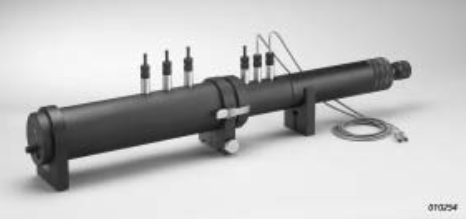
\includegraphics[width=0.7\textwidth]{Chapter-1/figs/impedancetube}
    \caption{Br�el \& Kj�r Impedance/Transmission Loss Measurement Tubes Type 4206A \cite{Kjaer2011}}
    \label{fig:impedancetube}
\end{figure}




